\documentclass[10pt,a4paper]{article}
\usepackage[utf8]{inputenc}
\usepackage{amsmath}
\usepackage{amsfonts}
\usepackage{amssymb}
\usepackage{graphicx}
\usepackage{url}
\usepackage{listings}

\usepackage{tikz}


\usepackage{color}

\definecolor{mygreen}{rgb}{0,0.6,0}
\definecolor{mygray}{rgb}{0.5,0.5,0.5}
\definecolor{mymauve}{rgb}{0.58,0,0.82}

\def\File#1{\textsf{#1}}
\def\Code#1{\texttt{#1}}
\def\Key#1{\textsf{#1}}

% Nice borders on matrices.
\usepackage{etoolbox}
\let\bbordermatrix\bordermatrix
\patchcmd{\bbordermatrix}{8.75}{4.75}{}{}
\patchcmd{\bbordermatrix}{\left(}{\left[}{}{}
\patchcmd{\bbordermatrix}{\right)}{\right]}{}{}

\parindent 0pt
\parskip 0.5\baselineskip

\lstset{ %
  backgroundcolor=\color{white},   % choose the background color; you must add \usepackage{color} or \usepackage{xcolor}
  basicstyle=\footnotesize,        % the size of the fonts that are used for the code
  breakatwhitespace=false,         % sets if automatic breaks should only happen at whitespace
  breaklines=true,                 % sets automatic line breaking
  captionpos=b,                    % sets the caption-position to bottom
  commentstyle=\color{mygreen},    % comment style
  deletekeywords={...},            % if you want to delete keywords from the given language
  escapeinside={\%*}{*)},          % if you want to add LaTeX within your code
  extendedchars=true,              % lets you use non-ASCII characters; for 8-bits encodings only, does not work with UTF-8
  frame=single,                    % adds a frame around the code
  keywordstyle=\color{blue},       % keyword style
  language=Octave,                 % the language of the code
  morekeywords={*,...},            % if you want to add more keywords to the set
  numbers=left,                    % where to put the line-numbers; possible values are (none, left, right)
  numbersep=5pt,                   % how far the line-numbers are from the code
  numberstyle=\tiny\color{mygray}, % the style that is used for the line-numbers
  rulecolor=\color{mygray},         % if not set, the frame-color may be changed on line-breaks within not-black text (e.g. comments (green here))
  showspaces=false,                % show spaces everywhere adding particular underscores; it overrides 'showstringspaces'
  showstringspaces=false,          % underline spaces within strings only
  showtabs=false,                  % show tabs within strings adding particular underscores
  stepnumber=2,                    % the step between two line-numbers. If it's 1, each line will be numbered
  stringstyle=\color{mymauve},     % string literal style
  tabsize=2                       % sets default tabsize to 2 spaces
%  title=\lstname                   % show the filename of files included with \lstinputlisting; also try caption instead of title
}

%TODO: The V model.

\begin{document}

\author{
  Ibrahim Nemli (s093477@student.dtu.dk)\\
  Søren Tidemand Møller Harving (s093472@student.dtu.dk) \\
  Kim Rostgaard Christensen (kroch@imm.dtu.dk)
}
\title{02241 - Robust software systems \\
	Final report
}

\maketitle

\begin{abstract}
A robust software system can be described as a system which aims to be unbreakable in several situations. Unbreakable does not mean that the system has not got any errors, but the errors that may occur are handled in a way, so that the system returns an understandable description of the error to the user, fails in a safe manner or possibly degrade to a lower level of functionality. However, robustness in general and indeed with regards to software is difficult to define and quantify.
\end{abstract}

\tableofcontents
\newpage
\begin{figure}[h]
\centering
\includegraphics[scale=0.4]{fig/dilbert_robust.png}
 \caption{The Dilbert take on robustness (License: grey area)}
 \label{fig:dilber_robustness}
\end{figure}


\section{Defining robustness}
As figure \ref{fig:dilber_robustness} states, robustness can be a fuzzy term which is sometimes over-sold by egar marketeers.
However, there exist several engineering disciplines that focus on robustness individually. The fields covered here are;
\begin{itemize}
\item Safety
\item Security
\item Resilience
\item Usability
\end{itemize}
While they are not mutually exclusive fields of engineering, they each have their own set of parameters to optimize.

\subsection{Safety engineering}

Seeks to optimize on factors that provide maximum safety, typically by focusing on the absence of errors or unsafe procedures. Safety can also be provided by the use of barriers which in general can be realized by, for instance, physical obstacles such as walls or fences, or merely regulations or safety standards (including legislations).
For the software world, barriers can be implemented by either coding standards, or language restrictions (e.g. sub-setting). Extensive testing is also applicable as it gives some confidence that a system is safe within the bounds of the test environment.

\subsection{Security engineering}

Is mainly concerned with the issue of keeping a system out of harms way by preventing malicious users (or programs) in misusing it.
Robustness in this meaning will be the absence of security breaches, strong authentication mechanisms and appropriate internal ACL’s\footnote{Access Control List}.
Security can be defined on numerous levels, from the hardware layer to the physical world - by hindering access to systems altogether.

\subsection{Resilience engineering}
Whereas safety engineering takes the high road of idealism, building systems that never breaks. Resilience engineering takes the low road of acceptance, embracing the fact that there are no perfect systems, or unsinkable ships to take an example.
The main parameter targeted for optimization here is fault tolerance, and the goal is to provide fault-tolerance and, where applicable, a fail-safe system.
In software systems, this is typically realized by adding redundant components or extra information to data\cite{KoKr07}
. This could be checksums/parities or validation schemas, such as DTD’s\footnote{Document Type Definition} for XML.

\subsection{Usability engineering}

Although not a robustness-specific field, more and more evidence suggest that bad and counter-intuitive human interfaces leads to bad decisions, which then again lead to system failures.
Usability engineering deals with what can be described as applied joint cognitive systems\cite{hollnagel2005joint} engineering, where the user interface of a system is not treated as a boundary layer, but more as a complete system \emph{containing} the human operator.
The goal is, in brief, to provide the right information, no more or less, at the right time to the user, and the appropriate methods of control.

\subsection{Summary}
Clearly, there are a lot of interests in improving the robustness of a software system, be the motivator either constant loss of data from word-processing application, or securing a nuclear power plant from melting down, everyone likes their software responsive, correct and robust.

\section{Programming principles}
\label{sec:programming_principles}

To help the programmer to build a robust software system, he or she can use the principles explained below.

\subsection{Programming defensively}

Programming defensively is one of the essential techniques in robust programming.
This is a method for ensuring that the software is functioning in every kind of unforeseeable usage of the program. In other words, we have to assume that the user wants to break the software by inserting any kind of absurd, incorrect or malformed inputs, which would cause an error in the program. In all those cases, the program should not be vulnerable for those kind of inputs. The program should be able to print verbose and reasonable error messages in which the user can react upon.
Even if there is a detailed documentation of how the program should be used, we cannot expect the user to have read it. If so we cannot ensure that, the user has fully understood the documentation.\\

It is difficult to write perfect code (maybe impossible) but you can take advantages of defensive programming in terms of improving the quality of the code. This will reduce the amount of bugs, since the source code has been written in such way that it behaves in a predictable manner despite all kinds of errors that could occur.
One could say that the aim in defensive programming is to reduce the amount of errors that could happen.

\subsection{Information hiding}

In this case, we have to hide data as much as possible and only give enough information which has been asked for.
This can be implemented by having well-defined interfaces through which the program can access the information needed.
In object-oriented programming languages, we have the term encapsulation. This is a technique for restricting the access to some of the object’s components. In this way we can make sure that none of the internal component for an object can be reached and manipulated from outside.
By hiding data as described above, we prevent users from manipulating data and in that way destroying other data intentionally which the users are not supposed to have access to.

\subsection{Assume the impossible}

In order to have robust software systems you have to take care of cases, which look like that never can happen, since they often will happen (e.g. in a different environment than the original environment where the code has been developed). Those cases are based on our expectation on how the program is going to be utilized and executed. If our expectations are not fulfilled regarding to the usage, then the program will crash. Therefore, the programmer may not omit to take care of those kinds of cases.
 
This is one of the most difficult concept to learn because it requires great knowledge of the scenarios where the program is going to be used.
Another perspective in this principle is that our code is not fixed. We have to know that the source code may be changed during maintenance or expanding its functionality. Those changes might affect other parts of the software, which may lead to impossible cases occurring. 

\subsection{Contract programming}
Contract programming is a more formal method for verifying the correctness of software.
The basic idea is that by adding additional semantics to your code, software tools can be used to prove whether or not a given procedure lives up to it's contract.
Consider the following prototype written in Ada using the SPARK annotation language:
\lstinputlisting[frame=single, language=Ada] {code_examples/Overflow_Example.adb}
The annotation specifies which conditions must be true upon entering the method (pre) and exiting (post). If we were to program the method so that X was decremented, or untouched, the verification software would fail and leave us with no option but to fix the bad implementation.
Contract programming is typically only used in safety-critical systems that mandates formal requirements for software correctness. Contracts and verification reports can be used as argument and documentation of the correctness of the software - according to specifications.

\subsection{The human-machine interface}
Considering that humans are considerably more error-prone than computers, it makes sense to build programs on the premises of human beings rather than the opposite. We can also see the, perhaps even inevitable, evolution from programming in binary to modern day textual/model-based programming as a direct effect of this.

\subsection{Software testing}
There are several ways to test software and some test methods suits the chosen development method more than others. To mention the most common test methods, we got test driven development, black and white box testing and unit testing.
To test the software does not prove that the code is correct, but it can be used together with code contracts as an argument for the correctness of the code.
When developing a system based on code contracts it does not make any sense to use test driven development. Instead the developer/tester can use white- and black-box testing or unit testing as an extension to the code contracts.
 
The goal of software testing is to find errors in a more systematic and effective way than just by doing randomly experiments or discover errors by accident when the program is being executed, thus software testing is crucial for ensuring robustness of the software.
 
The program might be syntactically well-formed and type-correct, but it can compute the wrong answer anyway. Those kind of errors (logical errors) is hard to deal with, since they cannot be found automatically, and it is our own responsibility to find and fix them.

There are many test techniques (such as acceptance test, sanity test, stress test etc.) but two of the most important techniques for testing the functionality of the software are white-box testing and black-box testing.
 
White-box testing is also called for structural testing and it is focusing on the internal structures of the program (program text). The tester constructs a collection of inputs and corresponding expected outputs that runs through all branches of the program that can be executed (if-then-else, while, for, switch, try-catch-finally, etc.).
 
Black-box testing, sometimes called external testing, focuses on the problem that the program is supposed to solve without looking into its internal structure. The tester constructs a test data set with inputs, which includes typical as well as extreme (maybe incorrect or malformed) input data and corresponding expected outputs.
 
Maybe it is impossible to make a perfect test or test everything (according to the resources available, time and money) and therefore there a good measure of a test’s comprehensiveness is code coverage.
There are many code coverage techniques; here we cover some of them:

\begin{description}
 \item [Method coverage] is a metric that measures whether every method were entered and executed at least once during execution time.
 \item[Statement coverage] measures whether the test has executed every statement of every method at least once time and which statements have not been executed. Statement coverage is typically achieved by the white-box technique, and it is often the best coverage one can achieve in practice.
 \item [Branch coverage] is a metric that measures which possible branches in flow control structures are executed. This can be done by recording the boolean expression in the  control structure evaluated to both true and false during execution.
 \item[Path coverage] aims to make sure that the test executes every execution-path through the program at least once. This is one of the techniques, which is usually impractical or impossible; since it can have infinite number of paths or some paths might be infeasible because some input data to the program under test can cause that particular path not being executed.
\end{description} 

\section{Applying the principles}
Reflecting on the principles stated in section \ref{sec:programming_principles}, the programming language Ada 2012 was chosen with the following motivation:

The main philosophy of Ada is \emph{strong} typing. It emphasizes the use of types, though self-defined types and numerous built-in types. Having strong typing in-language enriches the compiler with information which it can use to give the programmer feedback on potential overflows and type mismatches.

For instance, a classic example would be
\lstinputlisting[frame=single, language=Ada] {code_examples/date_example.adb}
Where we try to assign the variable \Code{Day} to a number that is outside of the defined range. This will trigger the following compiler warning;
\lstinputlisting[frame=single, language=make] {code_examples/date_example.output}
And raise the exception at run-time as predicted.

Another benefit, is that the model $\leftrightarrow$ code relationship can potentially be closer with appropriate types and constraints. E.g. your multiplicities can be asserted at compile time.

\subsection{Rules of engagement}
Besides the strong typing, Ada features a lot of both compile- and run-time rules and checks that serves as a safety mechanism - effectively preventing you from doing things like referencing a, perhaps deallocated, local object from a global scope for instance.

These rules exist both to protect the programmer from him/herself and to be able to make guarantees about the runtime stability.

\subsection{Parameter passing}
A strong feature of Ada is the way parameters for sub-routines are formalized. For starters, Ada distinguishes between functions and procedure, where a procedure is similar to a function returning void in other programming languages, and uses a \Code{in out} notation for parameters as opposed to specifying pointers/references/constant values. The philosophy here is that by showing your \emph{intent} with the parameters, the compiler can figure out how the actual passing should be done, warn about assignments to \Code{in} parameters and non-used \Code{out} parameters.

This also has the side-effect of not having to worry about pass-by-reference/pass-by-value, as this is now up to the compiler.

\subsection{Encapsulation}
There are several levels of encapsulation in Ada. The most common is the packages which have a specification part and an implementation part. These are separated into two distinct files with suffix \File{.ads} and \File{.adb} respectively. Only the parts exposed by the specification is usable outside of the package. This is similar to the header files from C.
Ada specifications can also have a private part, where types and subroutines can be applied restrictions; private types cannot be read, and private subroutines cannot be used outside of the package - except for child packages.
Package encapsulation rules are somewhat complex, and covered by the Ada Reference Manual (ARM) \cite{taft1997ada}.

\subsection{Contract programming and type invariants}
As of Ada 2012, contract programming is included as a language feature. It is enabled by compiling the program with the \Code{-gnatA} flag which enables assertions.
Contracts work by adding additional data to your declarations, and are enforced run-time like any other assertion. An example is shown in figure \ref{fig:ada2012_contract}
\begin{figure}[h]
\centering
\lstinputlisting[frame=single, language=Ada] {code_examples/ada2012_contract.ads}
 \caption{An example Ada 2012 contract.}
 \label{fig:ada2012_contract}
\end{figure}

Another new features is type invariants which asserts that a type is always consistent within the rules specified. The example in figure \ref{fig:ada2012_type_invariant} illustrates a network packet which must always have a valid CRC $\leftrightarrow$ payload relationship.

\begin{figure}[h]
\centering
\lstinputlisting[frame=single, language=Ada] {code_examples/ada2012_type_invariant.ads}
 \caption{An example Ada 2012 type invariant.}
 \label{fig:ada2012_type_invariant}
\end{figure}
\subsection{The human factor}
The language incorporates the philosophy ``programming as a human activity'' and generally encourages (or maybe even forces) you to be explicit in your code. A typical quote is that ``Ada usually favours the reader over than the writer''.
The compiler also works very hard to produce you with accurate information about where errors and warnings are locate, and possible remedial actions. It even detects minor misspellings.

\section{Project description}

\subsection{Analysis}
We are modelling the railway network as an undirected non-disjoint graph. The nodes of the graph are considered as stations and points (those that are not declared as station) and the tracks are considered as edges.
 
Each station has capacity for having at most one train visiting or stopping at the station at one time.
The tracks between two nodes is considered as single track (no double tracks between the stations). This means that there can only be one train moving from one station to another.  
 
All nodes must be connected to each other as a single connected component in order to confirm that the trains can reach from a node to all others.  A possible railway network could look like the graph seen in figure \ref{fig:graph}.

\begin{figure}[h]
\centering
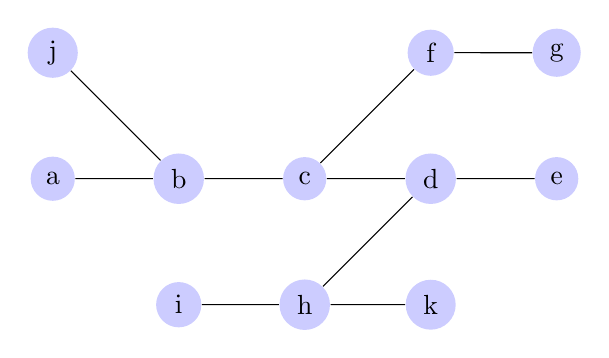
\begin{tikzpicture}
  [scale=.8,auto=left,every node/.style={circle,fill=blue!20}]
  \node (j) at (1,10) {j};
  \node (a) at (1,8)  {a};
  \node (i) at (3,6)  {i};
  \node (h) at (5,6)  {h};
  \node (b) at (3,8)  {b};
  \node (c) at (5,8)  {c};
  \node (d) at (7,8)  {d};
  \node (e) at (9,8)  {e};
  \node (f) at (7,10) {f};
  \node (g) at (9,10) {g};
  \node (k) at (7,6)  {k};


  \foreach \from/\to in {j/b, a/b, b/c, c/d, d/e, i/h, h/d, h/k, c/f, f/g}
    \draw (\from) -- (\to);

\end{tikzpicture}
 \caption{Example network}

 \label{fig:graph}
\end{figure}

\subsubsection{Simulation}
 
In order to keep the simulation simple the tracks have not been given any weights (e.g. a time unit moving on the tracks). Therefore, it takes one simulation time unit for a train to move from one node to another specified on its route.
 
Each train that has to be simulated has a route, which consist of a list of stations and points. The trains follows this route during simulation time. When the train arrives to the last station specified on its route, the train is then considered stopped at the station, and will appear there for the rest of the schedule lifetime.
 
\subsubsection{Train collision}
 
A train collision can occurs in two different situations:

\begin{description}

\item[Station collision:]
A train is collided on a station when two or more train arrives at the same station at the same time.
\item[Track collision:]
When two trains wants to cross each other e.g. a train moving from $a$ to $b$ while another train is moving from $b$ to $a$ at same time (keep in mind that we only have single tracks).
\end{description}

\subsubsection{Failure model}
For the purpose of determining the severity, we have defined a safety domain. This is basically just a 2-by-2 matrix that categorizes our different failure modes which are unsafe, but invalid routes and unsafe valid routes - where the latter is the critical one, and hence marked by red in figure \ref{fig:safety_domain}. Invalid routes \emph{can} be ignored, as they are unrealisable, but are convenient to know about during validation.

\begin{figure}[h]
\centering
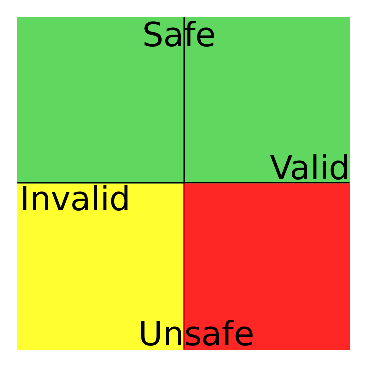
\includegraphics[scale=0.5]{fig/Safety_domains.eps}
 \caption{Basic model of the realm of our safety domain.}
 \label{fig:safety_domain}
\end{figure}
This is similar to a risk matrix, but simplified for the purpose of this assignment.

\subsection{Configuration}
 
We expect to read in two files. A file, which contains the configuration for the railway network and another, which contains the route for the trains.
 
\subsubsection{Railway network configuration}
 
This configuration consist of 3 (4, if count implicit declarations of tracks) parts; stations, connections and endpoints

\begin{description}
\item[Stations:] Stations are basically tracks with a string identification. It is formalized by ``\Code{STAT String ID}'' in the grammar, and thus serves as a station/id declaration and freezing.
\item[Connections:] Connections (CONN) are tracks and are formalized by ``\Code{CONN ID ID}'' in the grammar.
\item[End points:] Endpoints are track terminations.
\item[Non-station tracks:] These are characterized by by the absence of a station identification in a connection, and are thus not explicitly formalized in the grammar.
\end{description} 

As there is no requirements on the order in which \Code{STAT} and \Code{CONN} must appear, it is possible, from a parser point of view, to see a station before its declaration. In effect; a \Code{STAT} freezes the \Code{ID}, whereas a \Code{Conn} only marks it as defined.
 
Or more formalized;
\paragraph{Preconditions for stations:}
\begin{itemize}
  \item The station has not been created before (unique in terms of ID).
\end{itemize}

\paragraph{Post conditions for station:}
\begin{itemize}
\item The station becomes created as a node in the internal system.
\end{itemize} 

\paragraph{Preconditions for connections:}
\begin{itemize}
  \item The order of the ID’s does not matter e.g. CONN 2 4 is the same as CONN 4 2.
  \item An ID which is not declared as a station above is considered as a point.
\end{itemize}

\paragraph{Post conditions for connections:}
\begin{itemize}
  \item An edge has been created between two points or a point and an endpoint.
  \item ID which are not declared as a station above is created as a point in the internal system.
\end{itemize} 

\paragraph{Preconditions for end points:}
\begin{itemize}
  \item Only nodes with degree 1 can have endpoints (in the figure above: $j, g, a, e, i$ and $k$).
\end{itemize}
 
\paragraph{Post conditions for end points:}
\begin{itemize}
  \item End points are created in the internal system
\end{itemize}

\subsubsection{Route configuration}
 
Each route configuration read by the program correspond to a train that has to be simulated in the railway.
 
The trains can only change direction when they are stopped. This means that the \Code{ID} for time $T_i$ must be different than $T_{i+2}$, if $T_i$ is different from $T_i$ and $T_{i+2}$.
 
A route configuration as following: H L stop H or H L L H is considered to take the same amount of simulation time. A train can stop at all types of points (also for those that are not declared as stations).

\section{Design}
\subsection{Validation}
 
In order to have a valid railway network for simulation of the trains we are going to validate on three parameters before the simulation takes place:
\begin{enumerate}
\item Railway network validation: \\
      As described above the railway network must be connected to ensure connectivity and reachability from each node. This can be done by implementing the breadth-first search algorithm and check that it reaches every node in the graph. If it does not, then the graph is not connected as a single component and we can’t ensure that the given train routes are drivable based on the given network configuration.
 
\item Train routes vs. railway network validation: \\
      The routes must be drivable on the basis of the given network configuration. This should happen without jumping.
 
\item Trains routes validation: \\
      A validation regarding the train routes must ensure that the trains doesn’t collide during simulation time. 

\end{enumerate}
  
\subsubsection{Train routes}
 
The train routes are inserted in a matrix where the rows corresponds to train routes while the columns indicate the simulation time.
As an example of a configuration with three train routes would look like the matrix in (\ref{eq:sched1}).

\begin{equation}
M_{schedule} = \bbordermatrix{
                    ~ & t_0 & t_1 & t_2 & t_3 & t_4 \cr
                  r_0 & a   & b   & c   & d   & e\cr
                  r_1 & d   & c   & b   & a   & a\cr
                  r_2 & i   & h   & c   & f   & g}
\label{eq:sched1}
\end{equation}

A station collision is detected if a station/node is repeated two or more times for a given time (column).
In the example above, we can see that there is a station collision between route $r_0$ and $r_2$ for time $t_2$.
This check has to be done for each columns in the matrix.
 
A track collision is detected be looking for crosses such that for each row for time $t_i$ and $t_{i+1}$ there must not be a two stations in reversed order in another row.
An example of this is when train with route $r_0$ and the train with $r_1$ for time $t_1$ and $t_2$. ($r_0$ is moving from $b \rightarrow c$ and $r_1$ is moving from $ c \rightarrow b $) Here we can see that those trains wants to cross each other by moving on the same piece of track.  

In short; using this matrix, we can detect collisions using the following rules;

\begin{description}
  \item[RV1:] Each column must contain unique track identifications.
  \item[RV2:] For each column pair $\left( x_1,x_2 \right), \left( y_1,y_2 \right)$ the following must hold;\\ $\lnot\left(x_1 = y_2 \land x_2 = y_1\right)$.
\end{description}

\subsubsection{Enforcing rules}
For the purpose of checking uniqueness, we can use the abstract data type Multiset which fits the profile quite perfect, as it counts the occurrences of elements. 

We can detect violations of \textbf{RV2} using a type invariant.
\subsubsection{Optimizations}
\label{sec:optimizations}
 
The algorithm suggested for the track collision in the above section is quite slow since it has to check for each columns and rows. This algorithm has time complexity of: $O(n^2)$.
Therefore, we have suggested the following algorithm:
For each entry in the matrix above, we duplicate the content for each row such that we have the same station twice and then the concatenation with the next station. This duplication is done throughout the matrix. For the example above, the final matrix would look like (\ref{eq:sched2}).

\begin{equation}
M_{schedule} = \bbordermatrix{
                    ~ & t_0 & t_{0.5} & t_1 & t_{1.5} & t_2 & t_{2.5} & t_3 & t_{3.5} & t_4 \cr
                  r_0 & aa  &  ab     & bb  &  bc     & cc  &  cd     & dd  & de      & ee\cr
                  r_1 & dd  &  dc     & cc  &  cb     & bb  &  ba     & aa  & aa      & aa\cr
                  r_2 & ii  &  ih     & hh  &  hc     & cc  &  cf     & ff  & fg      & gg}
\label{eq:sched2}
\end{equation}

The entries in the matrix has to be ordered lexically so we can simply make string comparisons to detect uniqueness. And while we are at it, we adjust the time reference as well.

\begin{equation}
M_{schedule} = \bbordermatrix{
                    ~ & t_0 & t_1 & t_2 & t_3 & t_4 & t_5 & t_6 & t_7 & t_8 \cr
                  r_0 & aa  & ab  & bb  & bc  & cc  & cd  & dd  & de  & ee\cr
                  r_1 & dd  & cd  & cc  & bc  & bb  & ab  & aa  & aa  & aa\cr
                  r_2 & ii  & hi  & hh  & ch  & cc  & cf  & ff  & fg  & gg}
\label{eq:sched3}
\end{equation} 
Now we only have to look column wise. The columns should contain unique entries in order to have valid train routes.
A station collision is detected if there is duplicated entries for the even columns and a track collision is detected if there is duplicates in the odd rows.
 
The station collision in the previous example is now detected by the duplicate for route $r_0$ and $r_2$ in time $t_4$.
The track collection is detected by the duplication in $r_0$ and $r_1$ for $t_3$.
 
The optimized validation algorithm has time complexity of $O(2n-1)$, since the number of columns in the matrix has been roughly duplicated.

In effect, this eliminates the need for the second rule \textbf{RV2}, giving us only one thing to check, namely \textbf{RV1}.

\subsection{Optimizing train routes}
 
This part concerns possible optimizations that can be done on the train routes to avoid trains collisions to occur:
 
\subsubsection{Station collisions}
 
The program should avoid that trains collide with each other before those trains arrive at the same station/point. In order to avoid a station collision only one train is allowed to move while the other trains must wait. A possible way to implement this is to assign priority to the trains. If a train does not have to stop at the station concerned then this train has a higher priority than a train that has to stop. The computer picks up a randomly selected train with high priority and allow it to move while the others have to wait until there the station is available. As soon, there is no more trains with high priority waiting to pass the station, the lower prioritized trains will start to move.
With this solution, we could avoid trains blocking for others that just have to pass the station (remember that it takes one simulation time unit for stopping a train on a station).
 
\subsubsection{Track collision}
 
If this situation occurs, there is not much to do. A deadlock occurs since none of the trains can pass each other.
A rerouting of the train could be a possible solution but then the route might be significantly changed regarding the initial configuration setup. In some railway network configurations, it might not even be possible that such rerouting can take place.
 

\section{The V-model}
 
With the model we have the ability to change the view of point for the problems in the project.
For instance, this model could be used in the case of validating the network. Instead of checking the network configuration makes a valid network, we know that it should be possible to create a graph, which is a subset of the original graph on the basis of the matrix which contains the train routes. This graph might be
a disjoint graph, but this would indicate that some of the tracks are not used in the system.
\begin{figure}[h]
\centering
\includegraphics[scale=0.6]{fig/user_interface.png}
 \caption{User interface}
 \label{fig:user_interface}
\end{figure}

To visualize the output on how the network of the tracks looks like and how the different route are scheduled compared to each other over time, the following will be used as part of the output. 
The right side of the picture depicted at figure \ref{fig:user_interface} shows the network, based on stations and tracks. The left side of the picture shows how the routes overlaps on $t\left(n\right)$.


\section{Implementation}
\subsection{Testing}
\subsubsection{Route and schedule validator}
Due to the implementation of two independent modules, each module has been test separately.
Network and Route Parser
This part of the system is tested mainly by black-box testing. Several cases, input files, has been made, mostly containing errors, and the output has been examined. To make the tests cover more areas, the cases has been written by different people.
The test cases are listed in the appendix A and B.
Three cases fails; 11,12 and 13. This is caused by two things; 
\begin{itemize}
  \item The validator does not couple the networks with the schedules, as this was not needed to ensure the safety and correctness of them individually. Our focus was on safety, and absence of collisions.
  \item The route validator does not check for disjoint networks. This is an error, and should be fixed in a later revision.
\end{itemize}

The full result of the tests can be found in appendix A.

\subsection{Simulator}
This section contains test cases (black-box) and test results which has been made for the railway simulator. 
The test has been separated in three different categories, each having its own aim for ensuring the robustness of the railway simulator software tool. 
The first test has focused on the validation of the routes before the simulation takes place. During this test, we had one railway configuration and changed the route configuration with different test parameters. The results of the different tests can be found in appendix B.

The next test focuses on the validation of the railway network configurations. During this test, we have changed the railway configuration with different test parameters. The results of the different tests can be found in appendix C.

The railway simulator tool does not check how many tracks is connected to a station or point there test 2.6 fails. This is not implemented! 
In the final test for the railway simulator, we have as input given an invalid railway network configuration (a disjoint graph) together with a valid route configuration.
The results of this test is found in appendix D.

The reason for the fail in test 3, is that there is no implementation of an algorithm which checks that the graph is disjoint.

\subsection{Railway simulator}
The implementation architecture for the railway simulator is quite simple. A class diagram for the software is shown on the figure below.
A Main class is used to initialize a VisualizationPanel class. This class is responsible for parsing the input files and create three other panels ScheduleGraph, NetworkGraph and StatusPanel.
 
The Parser class reads the railway network configuration file and the route file. When those files are read line by line, the different check methods are run in order to confirm the validity of the files (see methods in the Parser class). If no errors are found proper domain objects are created. These objects are given to the panels to simulate the routes on the railway system.
 
The first panel created is the ScheduleGraph. It creates a xy-chart, which draws the routes such that you can see where the trains are located in the railways system for a given timestamp.
This panel is interactive such that the timestamps are clickable. A click on a timestamp will look for station and track collisions based on the current train information (traffic).
If any collisions are detected it is written on the StatusPanel. This panel is used for prompting textual information to the user. 
 
The NetworkGraph panel is used for visualize the railway network as a graph (using the JUNG framework).
In addition, this graph is also used to show collisions occurring in the railway system.  

\begin{figure}[h]
\centering
\includegraphics[scale=0.5]{fig/uml.pdf}
 \caption{UML diagram of the simulator}
 \label{fig:uml_simulator}
\end{figure}

\subsection{Route validator}
The route validator is implemented as a light-weight compiler. I has a tokenizer that generates a ``fat token'' containing an abundance of information. Based on the identity of these tokens, they are dispatched to various handlers that are coupled to a route object.
When no more input (end of file) is detected, we validate by freezing each rail. The freeze operation merely casts the \Code{Rails} object to a \Code{Frozen\_Rails} object, which is just a subtype of \Code{Rails}, but with a type invariant - effectively giving us a check for validity of each node.
\subsection{Schedule validator}
This tool has a more crude parser (without the tokenizer), and converts the schedules to our internal format as described in section \ref{sec:optimizations}. From hereon we validate each column by enumerating each occurrence in a multiset. Upon failure, we raise a \Code{Train\_Collision} exception - which give out more information about what went wrong.

\section{Usage}
\subsection{Route validator}

\subsection{Schedule validator}
This user guide describes to how to use the program. The guide consist of two parts. The first part is concerned about the validation software for the network and route configuration file, where the second part is concerned about the railway simulation program.
This guide will quickly let you begin to use the software.

\subsubsection{Network and schedule validation tool}
 
This part consists of two programs that both should be run for a complete validation. A network parser and a route parser.
The network parser will validate a specific network file for any errors. The output will be a prompted text message in the command prompt. The same goes for the route parser.
If the network parser reports any errors, these should be corrected before running the route parser.

\begin{itemize}
 \item 
\end{itemize}
The schedule validator is a command line tool that takes in single argument, which is a file path for a schedule file. Upon completion the program either outputs the text Schedule ``is valid'' or "Schedule is invalid, followed by a description on what errors are detected. An example of this is shown below.
\lstinputlisting[frame=single, language=make] {code_examples/schedule_validator.output}

The route validator is also a command line tool that takes in single argument, which is a file path, but this time for  a route file.
The console will prompt any errors or tell you if it is validated successfully

If everything is validated successfully, fell free to use the simulator tool to see how the network is created and how the trains are scheduled
The visualizing tool can also be used to see any network or schedule errors.

\subsection{Simulator}
Railway simulation software tool

The railway simulation program starts from the command line. Please open the command line and type in following command from the path where the file RailwaySimulation.jar is located:

\Code{java -jar RailwaySimulation.jar networkfile rutefile}\\
 Replace \Code{networkfile} and \Code{rutefile} with the name of your network configuration and route configuration files
 
\Code{java -jar RailwaySimulation.jar net1.txt rute1.txt}

If no errors found in the given files, the program will now open a graphical user interface. Otherwise, you will be prompted an error message on the console. Please correct those errors and restart the program (example on errors: no track between two stations, no files found, syntax errors in configuration file, no station/node detected etc.).
 
The graphical user interface consist of three panels:
The upper left panel is the train scheduling. Next to this panel is the network panel found. At the bottom, the status panel is located.

\subsubsection{Train scheduling panel}
This panel maps the routes from the route configuration, and shows where the trains are for a given time on a coordinate system.
 
Click on the time labels (starting from t0) and it will color the nodes on the network panel indicating where the trains are for the given time on the network panel.
If a collision is detected this will be written in the status panel and be indicated on the graph.
 
Indications of collisions on the train scheduling panel:
\begin{itemize}
  \item When a station collision is detected, two or more routes will intersect at the same station.
  \item When a track collision is detected, and symmetric cross will be found in the column between the time stamp clicked, $t_{clicked}$ and $t_{clicked - 1}$.
\end{itemize} 

Examples of the two cases are shown in figure \ref{fig:graphical_schedule}
\begin{figure}[h]
\centering
\includegraphics[scale=0.7]{fig/visual_graph.png}
 \caption{Station collision at Lyngby at $t_5$ and track collision at $t_4$ and $t_5$ between Farum and Bagsværd shown on the train scheduling panel}
 \label{fig:graphical_schedule}
\end{figure}

\subsubsection{Network panel}
 
This network panel shows the railway network configuration modelled as an undirected graph (stations/nodes as nodes and tracks as edges).
 
The graph (GUI) provides two modes: translate (pan) mode and picking mode. You can change to translate (pan) mode by typing ``t'' and to picking mode by typing ``p''.
Different modes gives activates different functionalities:
 
Functionalities in translate (pan) mode:

\begin{enumerate}
  \item Left mouse click and mouse drag in the graph window allows you to translate (pan) the graph.
  \item Shift, left mouse click and drag in the graph window allows you to rotate the graph.
  \item Control, left mouse click and drag in the graph window allows you to shear the graph.
  \item Mouse wheel or equivalent allows you to scale (zoom) the graph.
\end{enumerate} 
Functionalities in picking mode:
 
\begin{enumerate}
  \item Left mouse click and mouse drag on a node allows you to move the node.
\end{enumerate}
 
Indications of collisions in the network panel:
 
When a station collision is detected, the node concerned becomes red.\\
When a track collision is detected, the edge on the graph becomes red.
 
Examples of the two cases are shown in figure \ref{fig:collision}.

\begin{figure}[h]
\centering
\includegraphics[scale=0.7]{fig/collision.png}
 \caption{Station collision at Lyngby and track collision on track between Farum and Bagsværd shown on the network panel}
 \label{fig:collision}
\end{figure}
 
This panel prompts status messages when collisions occurs. Right click on this panel provides you following features:

\begin{enumerate}
  \item Clear panel: clears the text on the status panel.
  \item Clear graph: resets the colors of the graph (to default white)
\end{enumerate} 

Indications of collisions in the status panel:
 
When a station collision is detected, it will be written on the status panel.
When a track collision is detected, it will be written on the status panel.
 
Examples of the two cases are shown in the figure \ref{fig:status panel}.

\begin{figure}[h]
\centering
\includegraphics[scale=0.7]{fig/status.png}
 \caption{Status panel}
 \label{fig:status panel}
\end{figure}

\section{Conclusion}
\subsection{What is robustness?}
\begin{quote}
\textit{- It is a burden, hard to fulfil, can be confusing and simply just a pain in the ***.}
\end{quote}

The term ``robust’' is, despite the hard attempt to define it, still difficult to define precisely. Therefore it becomes something abstract that the programmer must think about in the analysis/design and implementation phase. The project together with the lectures has given us an insight on which elements to be aware of in software engineering that has high demand and requirements on robustness.
Keeping the three robustness principles, programming defensively, information hiding and assume the impossible, in mind when developing a software system has shown to come in handy. It makes you think of what can happen with data when a user calls a method. Also how to avoid the user from ``breaking the method'' by making the method to return unexpected values or even make the system crash.
By using Ada 2012 we are provided with an easy access to handle this. You don’t
have to rely on an external verification compiler like SPEC\#, because it is already a part of the language. The language itself is not similar to C\# as C\# is to Java, C++ etc. You have to spend some time learning the basics of the language, which can be quite a challenge, compared to learning C\# if you already know Java. But with that being said it is very easy to implement the type invariants and pre- and post-conditions discussed during the design phase.

\subsection{Now what is robustness?}
- Something that every developer should keep in mind when designing and writing code and it really pays off in the end, both for the developers and the users: Defensive programming and defensive design.

\subsection{The course}
Trying to build a more formal proof of small and simple to verify building blocks to argue for the correctness of the complete system has been a great learning experience for us. The approach of making unsafe conditions a contradiction to the logic is very intuitive and makes the validation process very iterative. For the course in general, the what-ifs proposed by the instructor has given a lot of food for thought. Especially the talk about interfacing, with regards to LLVM, made us reflect on the importance on protocols and clear descriptions for interfaces.
We also really enjoyed the talk from Software Improvement Group, which gave a good birds-eye perspective on the quality of, and metrics for software.

% The following two commands are all you need in the
% initial runs of your .tex file to
% produce the bibliography for the citations in your paper.
\bibliographystyle{plain}

% These are entries that should be a part of references, no matter if they were cited or not.
\nocite{Dijkstra:1979:PCH:1241515.1241516}
\nocite{Chapman:2006:CCM:1151816.1151820}
\nocite{bishop2004teaching}
\nocite{Wikipedia:Defensive_programming}
\nocite{Wikipedia:OO_encapsulation}
\bibliography{references}  % sigpr

\end{document}